\documentclass[../dissertation.tex]{subfiles}

\begin{document}

\subsection{Experiment 1 - Revising Existing Code}
\label{exp-1}

\paragraph{Introduction} To begin, initial testing of ROS' communication ability must be carried out - meaning that before further investigation can be done, one must understand what baseline performance one can expect from ROS on the hardware platform used. A useful example is the need to identify an order of magnitude estimate for the message frequency (messages per second) we can expect from ROS. A network architecture must also be worked out that allows for repeatable and accurate measurements of inter-robot communication performance.

A prior investigator, Andreea Lutac\cite{andreeaLutacBlog}, had began investigation of building a simple experimental environment - however the results were not as expected. The architecture created by Andreea involved three robots (or hosts), the master host would simply run the ROS Master node providing name resolution services to the other two nodes as described in Section \ref{background-ros}. The sender host would contain a single ROS node that performs two tasks: sending a message containing a unique message identifier (ID) and a timestamp indicating the system time on the sender host the message was sent at, the second task would be to listen to responses from the third node. The third node is an echoer node which listens for messages sent from the sender, and simply sends them back. When the sender receives a message from the echoer, it again notes it's system time, and then writes message ID, sent time, and received time to disk - for later analysis. However, as mentioned earlier, the results were unexpected and unexplainable - the exact nature of which will be seen in the results section.

\paragraph{Objective} The aim of the experiment was to analyse the transfer time of messages between two machines at varying message frequencies, and identify whether there was some limit as to how often ROS could send and receive messages on it's topics. The experiment therefore had several objectives. First, repeat Andreea's experiment using the same code\cite{Experiment1InitialCode}, and verify the results were not due to a configuration error of the system. Second, to provide familiarity with ROS and grasp an understanding of how ROS communication works. And third, identify the underlying cause of the unexpected results and either analyse why ROS exhibits this behaviour or identify possible errors in the experiment code that would cause counter-intuitive results.

\paragraph{Hypothesis} The expected result of the experiment was that message latency would be the same across all lower frequencies - until some bottleneck in the system was reached. It is expected that once a bottleneck is reached that message latencies would increase exponentially due to congestion (i.e. messages would be being generated faster than the system could process them, causing an increasing number to be left waiting in message queues).

\paragraph{Materials and Methodology} The hardware set-up of this experiment was designed to isolate the system being tested from as many external variables as possible. The three host machines used were all Raspberry Pi 3 Model Bs freshly installed with the latest available stable version of the Raspbian OS (the official operating system for Raspberry Pis), and the latest available stable version of ROS (Kinetic). The Raspberry Pis were powered with a stable 5V power supply connected to the building's mains power. Each Pi was connected to a gigabit-capable Asus router via an Ethernet cable. The router was dedicated to the experiment, meaning that it had no other hosts connected to it other than the three Raspberry Pis and a Ubuntu desktop machine for controlling and monitoring of the Raspberry Pis. The Raspberry Pis had no peripherals (e.g. mouse, keyboard, camera, etc) connected, and were controlled via SSH connections.

As mentioned in the experiment introduction, the code base utilised to begin this experiment was previously developed\cite{Experiment1InitialCode}, and involved three Raspberry Pis: a master, a sender, and an echoer. The master simply allows the sender and receiver to contact each other. The sender generates messages containing a message ID, a sent timestamp, and a payload - in this case, a simple `Hello World' string - and sends them to the echoer. The echoer repeats any received message back to the sender exactly. Upon receiving the echo the sender then notes down message ID, sent time, and received time in a log file. This architecture is outlined in Figure \ref{exp1-architecture}, although the master node is omitted for clarity.

\begin{figure}[h]
\centering
\includegraphics[width=\textwidth]{images/experiment1/Experiment1-Architecture.png}
\caption{Experiment 1 - Communication Architecture}
\label{exp1-architecture}
\end{figure}

\begin{figure}[H]
\centering
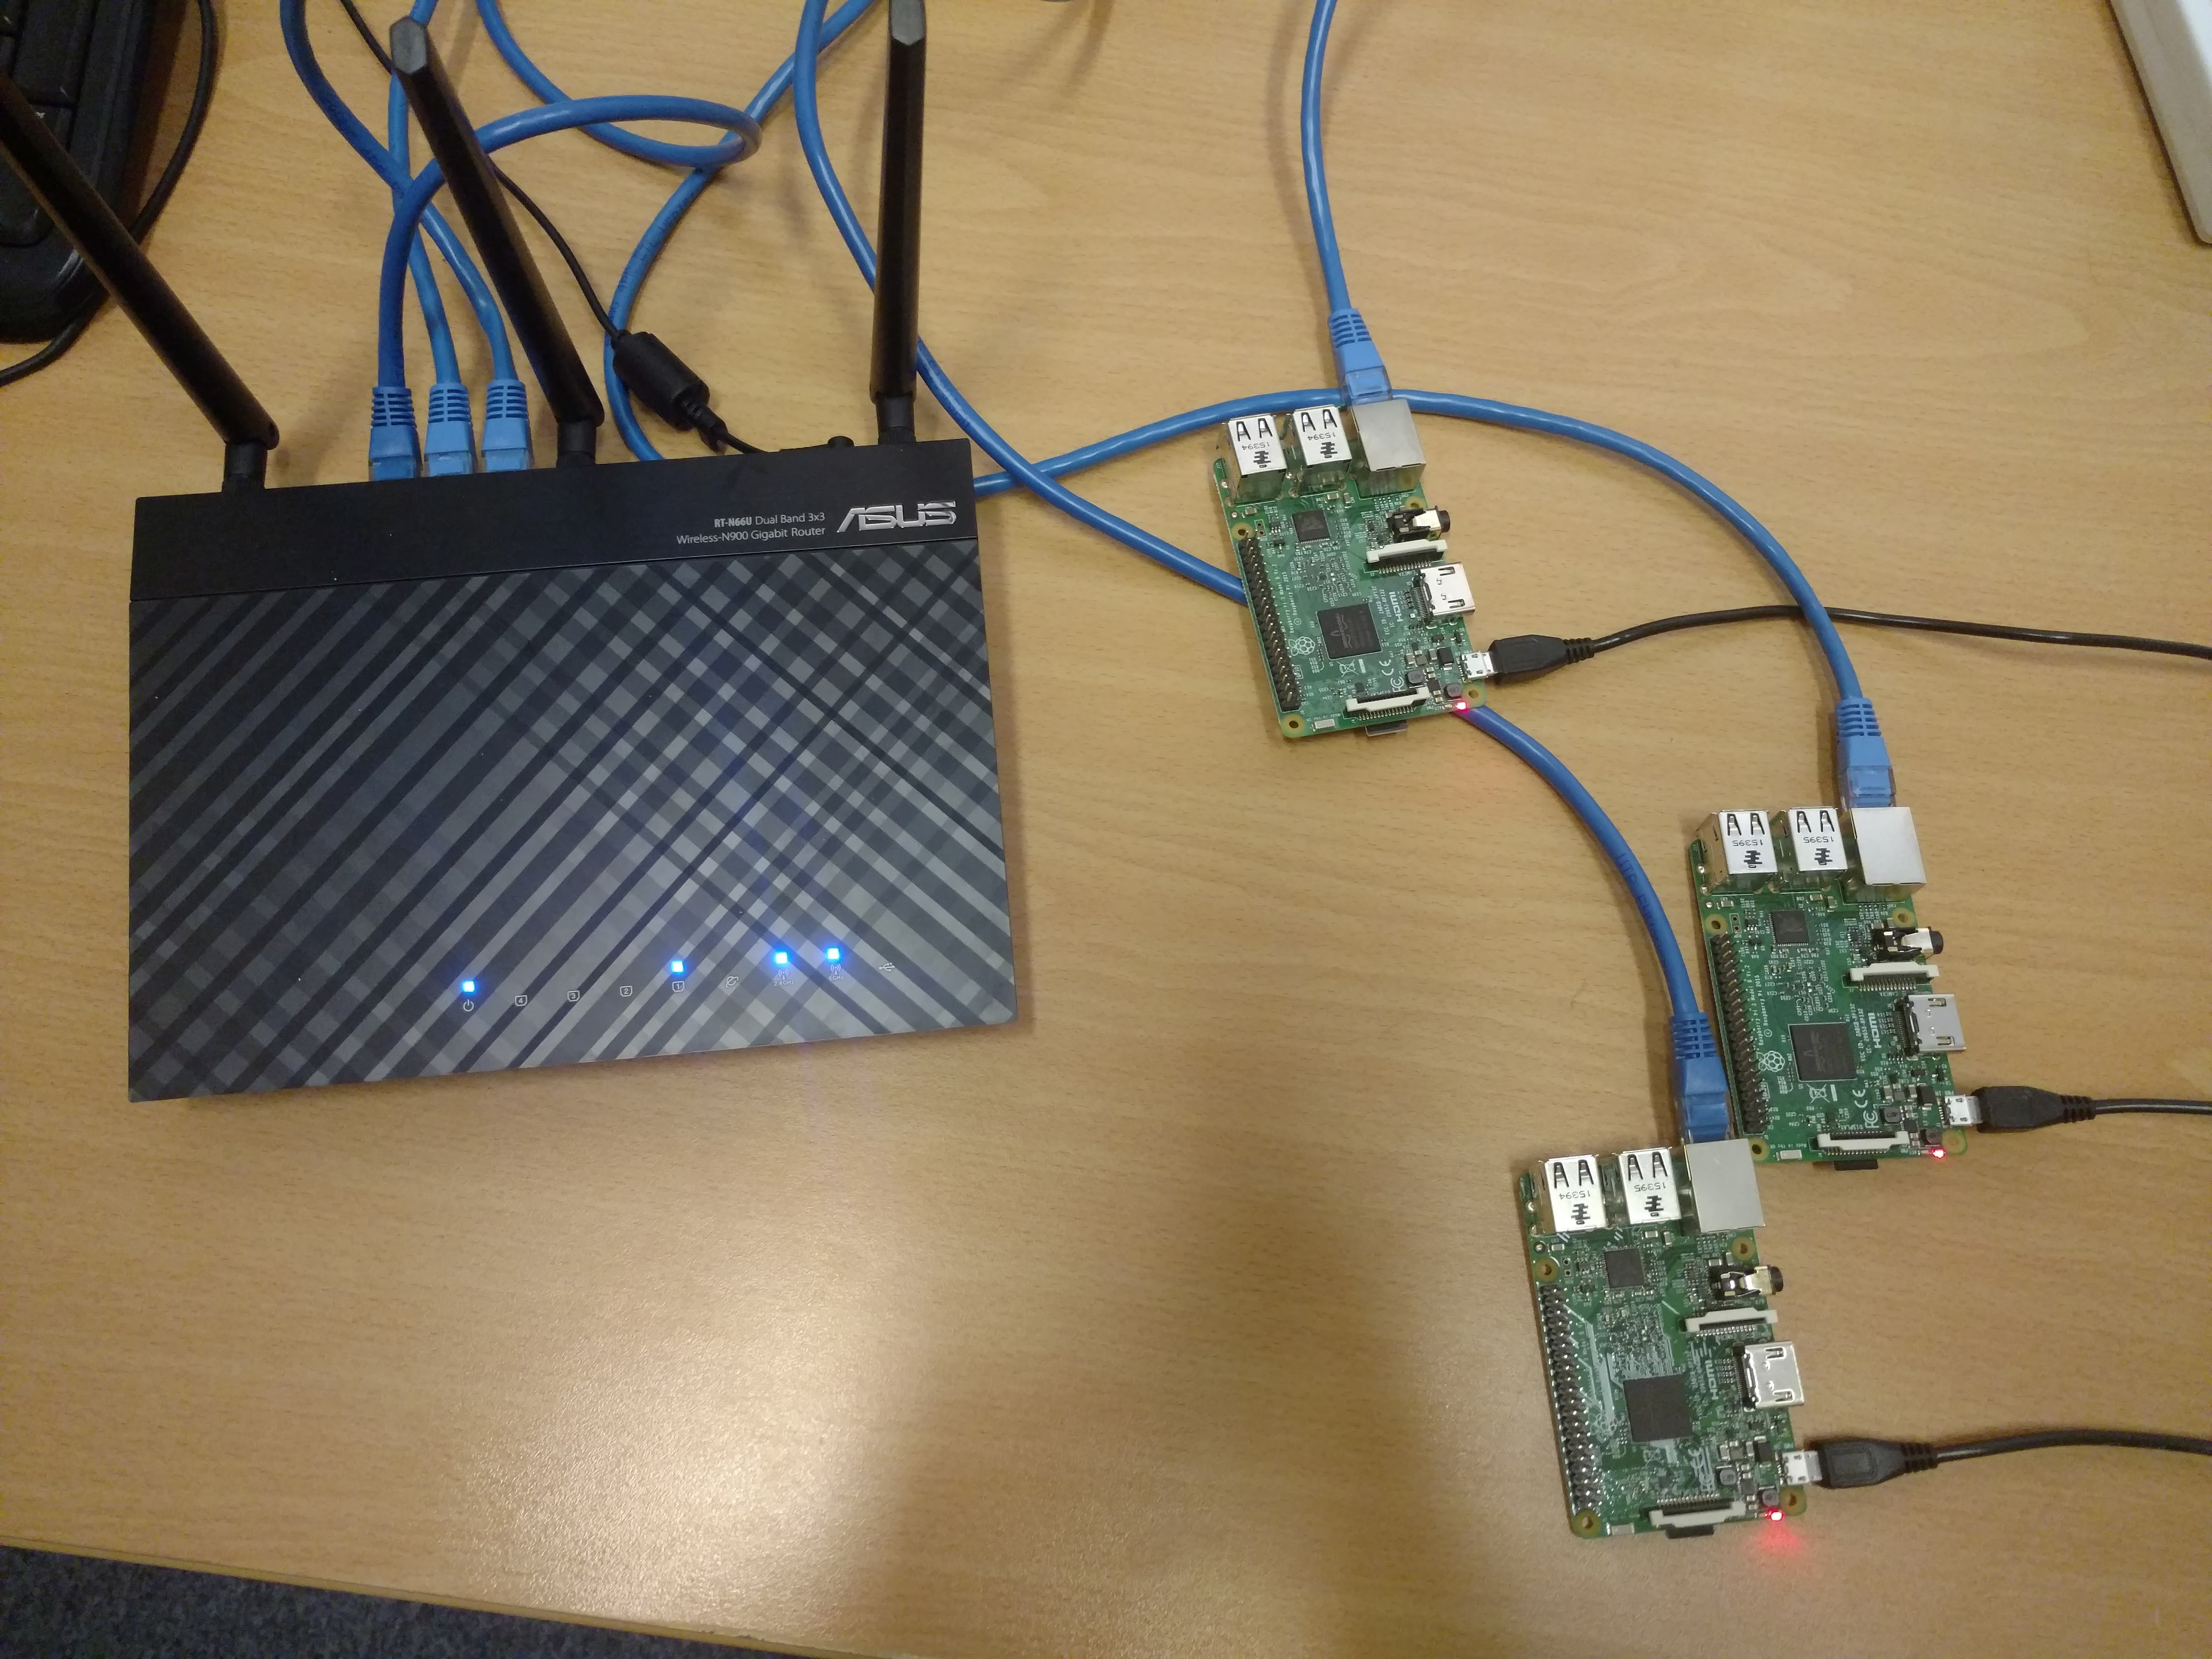
\includegraphics[width=0.7\textwidth]{images/experiment1/bare-pis.jpg}
\caption{Photo of the three Raspberry Pi Model Bs and Asus router utilised in Experiment 1}
\end{figure}

%The experimental setup was that one Raspberry Pi would run a ROS master node, another Raspberry Pi runs a sender program that notes down the message-sent time, and sends it to a 3rd Raspberry Pi which merely echoes the message back to the sender. Upon receiving the message, the sender/receiver notes the current time, and writes `message X which was sent at Y, was received at Z' to a text file. The resulting Round Trip Time (RTT) for each message would therefore be the difference between the message-sent time and the message-received time.

%Code had been written prior to execute this experiment, so initially this was used\cite{Experiment1InitialCode}. However, this gave results that were contrary to the hypothesis. An increase in message frequency resulted in a reduction in message latency. A number of messages on higher frequencies were also dropped, and never received. As this was the opposite of the hypothesis, the first step was to critique the experiment code.

\paragraph{Results and Discussion} This set-up was coded and ran, however as mentioned, the results were unexpected - as Figure \ref{exp1-all-freqs}, the set-up gave results that were contrary to intuition. As the sending message frequency increased, better performance (lower message latency) was seen - although at very high frequencies a number of messages were completely dropped at the start. These correlations can be seen in Figure \ref{exp1-all-freqs}. \textit{The results matched what was previously seen by Andreea - which directly conflicts with the hypothesis that increasing message frequency would eventually increase message latency.} Another interesting observation is that for 10KHz the first 169 messages were completely dropped (never received back from the echoer), and for 1MHz the first 312 messages were dropped. Figure \ref{exp1-dropped-messages} shows the total number of messages received for each frequency. \textit{These dropped messages indicate that the publisher message queues for either the sender or the echoer reached max capacity (causing some messages to be overwritten before they are sent)}.

\begin{figure}[H]
\centering
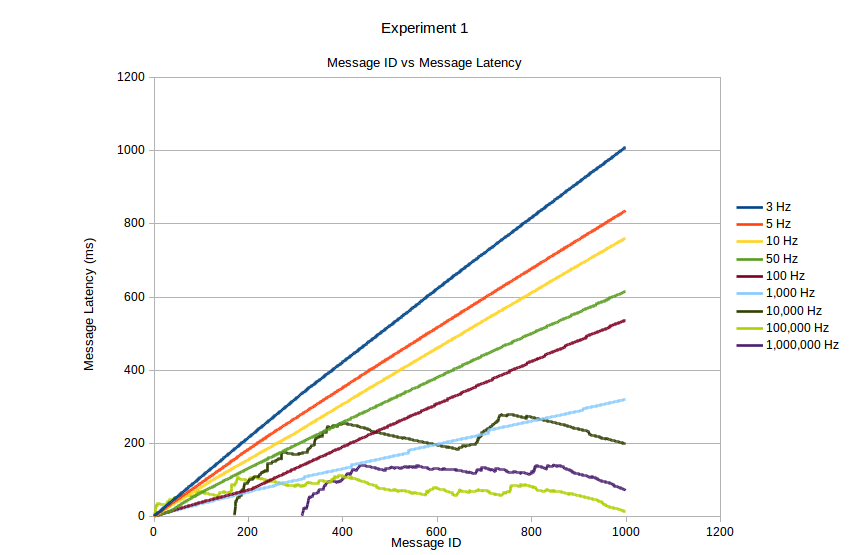
\includegraphics[width=\textwidth]{images/experiment1/msgid_msglatency_all_freqs_version_1.png}
\caption{Experiment 1 - Message Latency by Message Frequency}
\label{exp1-all-freqs}
\end{figure}

\begin{figure}[H]
\centering
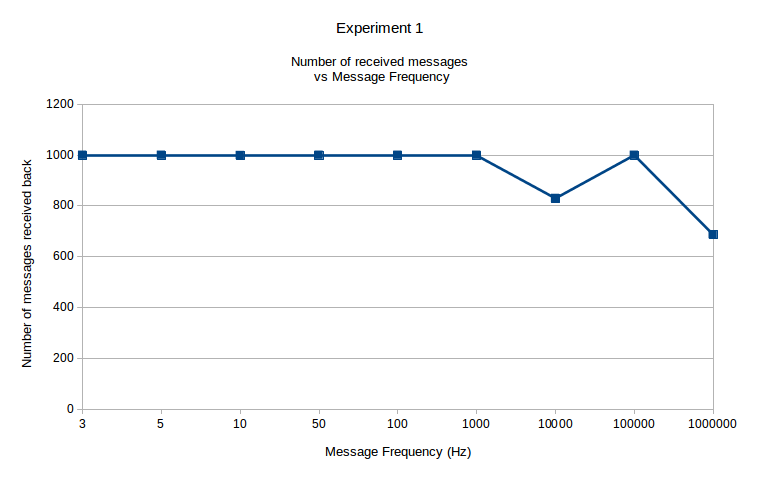
\includegraphics[width=\textwidth]{images/experiment1/original-messages-dropped.png}
\caption{Experiment 1 - Number of Messages Received by Message Frequency}
\label{exp1-dropped-messages}
\end{figure}

The next objective was to identify why these results were not as expected. The first step was to review the code being used to run the experiment, and try to identify any code that could cause anomalous behaviour. While conducting this review, two major issues were identified. The first was the echoer code had a delay similar to the sender when the experiment design mandated that the echoer always respond as fast as it can - so that only time taken to send the messages back-and-forth is measured. The second issue was the the maximum message queue size in ROS (how many messages can be buffered at once to compensate for a slow subscriber) was set equal to the message frequency of that run.

\begin{lstlisting}[language=Python, caption=Echoer Original]
import rospy
from rosberry_experiments.msg import StampedMessage
import time
import sys

RATE = None

def listener(msg, args):
    rate = rospy.Rate(RATE)
    pub = args[0]
    pub.publish(msg)
    rate.sleep()

def main():
    global RATE
    RATE = int(sys.argv[1])
    try:
        rospy.init_node('talker1', anonymous=True)
	      pub = rospy.Publisher('chatter_s', StampedMessage, queue_size=RATE)
        sub = rospy.Subscriber("chatter_m", StampedMessage, listener, callback_args=[pub])
		    rospy.spin()
    except rospy.ROSInterruptException:
        pass

if __name__ == '__main__':
	  main()
\end{lstlisting}

These issues were resolved by removing the code that executed the delay in the echoer, and by setting the maximum queue size to be equal to 1000 in every experiment (the number of messages expected to be sent). These modifications can be seen in Listing \ref{exp1-modified-listing}.

\begin{lstlisting}[language=Python, caption=Echoer Modified, label={exp1-modified-listing}]
import rospy
from rosberry_experiments.msg import StampedMessage
import time
import sys

def listener(msg, args):
    # No longer waits after receiving a message
    pub = args[0]
    pub.publish(msg)

def main():
    N = int(sys.argv[2])  # Total number of messages expected (1000)
    rospy.init_node('talker1', anonymous=True)
    pub = rospy.Publisher('chatter_s', StampedMessage, queue_size=N)
    sub = rospy.Subscriber("chatter_m", StampedMessage, listener, callback_args=[pub])
    try:
        # Wait until interrupted
        rospy.spin()
    except rospy.ROSInterruptException:
        print "Exception: ROSInterruptException"

if __name__ == '__main__':
    main()
\end{lstlisting}

The experiment was then repeated using this new echoer code. Figure \ref{exp1-modified-all-freqs} shows the message latency for each message at all frequencies. All frequencies less than 10KHz had concistent message latencies around 1.5ms, but 10KHz, 100Khz, and 1MHz exhibited very erratic performance - indicating that beginning around 10KHz the system begins experiencing a bottleneck. Figure \ref{exp1-modified-mean-latency-all-freqs} shows mean latencies across the entire message streams for each frequency - \textit{clearly demonstrating that performance is very consistent up until 10KHz for this set-up}.

\begin{figure}[H]
\centering
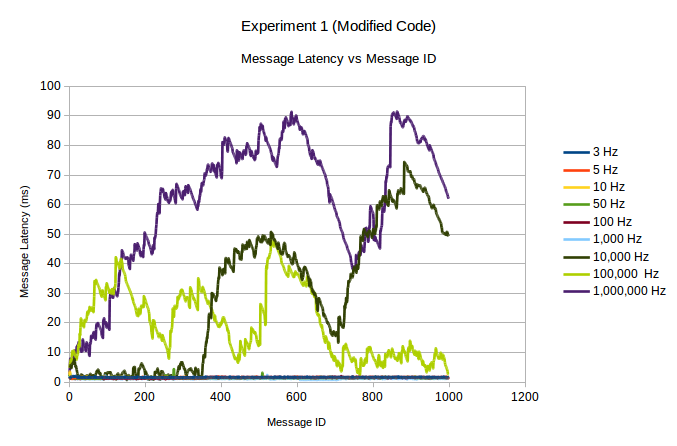
\includegraphics[width=\textwidth]{images/experiment1/modified_msgid_msglatency_all_freqs.png}
\caption{Experiment 1 (Modified Code) - Message Latency by Message Frequency}
\label{exp1-modified-all-freqs}
\end{figure}

\begin{figure}[H]
\centering
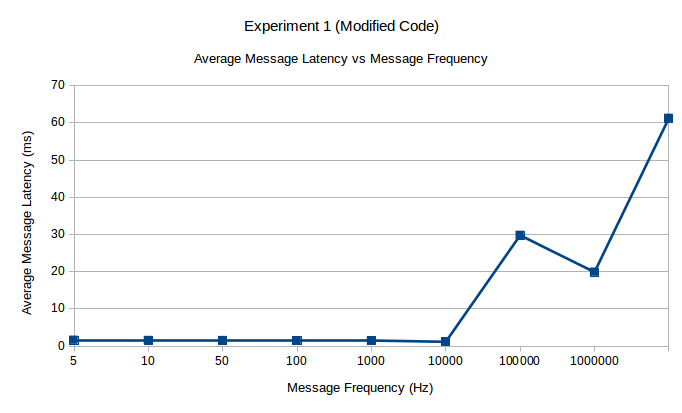
\includegraphics[width=\textwidth]{images/experiment1/modified_average_msglatency_all_freqs.png}
\caption{Experiment 1 (Modified Code) - Mean Message Latency by Message Frequency}
\label{exp1-modified-mean-latency-all-freqs}
\end{figure}

\subsubsection{Disk Writing}

At this point it was theorized that writing the results to disk during the experiment (as the sender receives messages back from the echoer) could be adversely affecting the performance at high message frequencies. Thus, an informal experiment was conducted to investigate if it was feasible to postpone writing the records to disk until the end of the message stream. This was coded, however unexpectedly gave rise to significantly higher message latencies. It is presumed this was an issue with the implementation - but it was then noted that Python uses the operating system's buffering mechanic to efficiently write to disk in blocks. \textit{Thus this idea was discarded, as it not expected that saving writing to disk until the end would be significantly faster than the buffering provided by Linux.}

\end{document}
